\documentclass{article}
\usepackage[margin=1in]{geometry}%设置边距,符合Word设定
\usepackage{ctex}
\usepackage{setspace}
\usepackage{lipsum}
\usepackage{graphicx}%插入图片
\usepackage{subcaption}
\usepackage{multirow}
\graphicspath{{Figures/}}%文章所用图片在当前目录下的 Figures目录

\usepackage{hyperref} % 对目录生成链接,注:该宏包可能与其他宏包冲突,故放在所有引用的宏包之后
\hypersetup{colorlinks = true,  % 将链接文字带颜色
	bookmarksopen = true, % 展开书签
	bookmarksnumbered = true, % 书签带章节编号
	pdftitle = Week2 Experiment Summary, % 标题
	pdfauthor =Ali-loner} % 作者
\bibliographystyle{plain}% 参考文献引用格式
\newcommand{\upcite}[1]{\textsuperscript{\cite{#1}}}

\renewcommand{\contentsname}{\centerline{Contents}} %经过设置word格式后,将目录标题居中


\title{\heiti\zihao{2} 实验小结}
\author{\songti Wang Yunyi}
\date{2025.10.01}


\begin{document}
	\maketitle
	\thispagestyle{empty}

%\tableofcontents

\section{实验}
实验对象共有4个,分别为:基础MLP模型(MLP),小型CNN模型(SmallCNN),参考ResNet思路并加入了残差块的CNN模型(ResCNN),简化版ResNet18模型(SmallResNet)。

设置EarlyStopping的patience为7,最大epoch数为32,所有生成随机数的种子均为608,使用AdamW优化器和CosineAnnealingLR,其他超参数均保持相同,位于config.yaml中。经过训练,4个模型在训练集、验证集上的的准确率和损失如图1。
\begin{figure}[htbp]
	\centering
	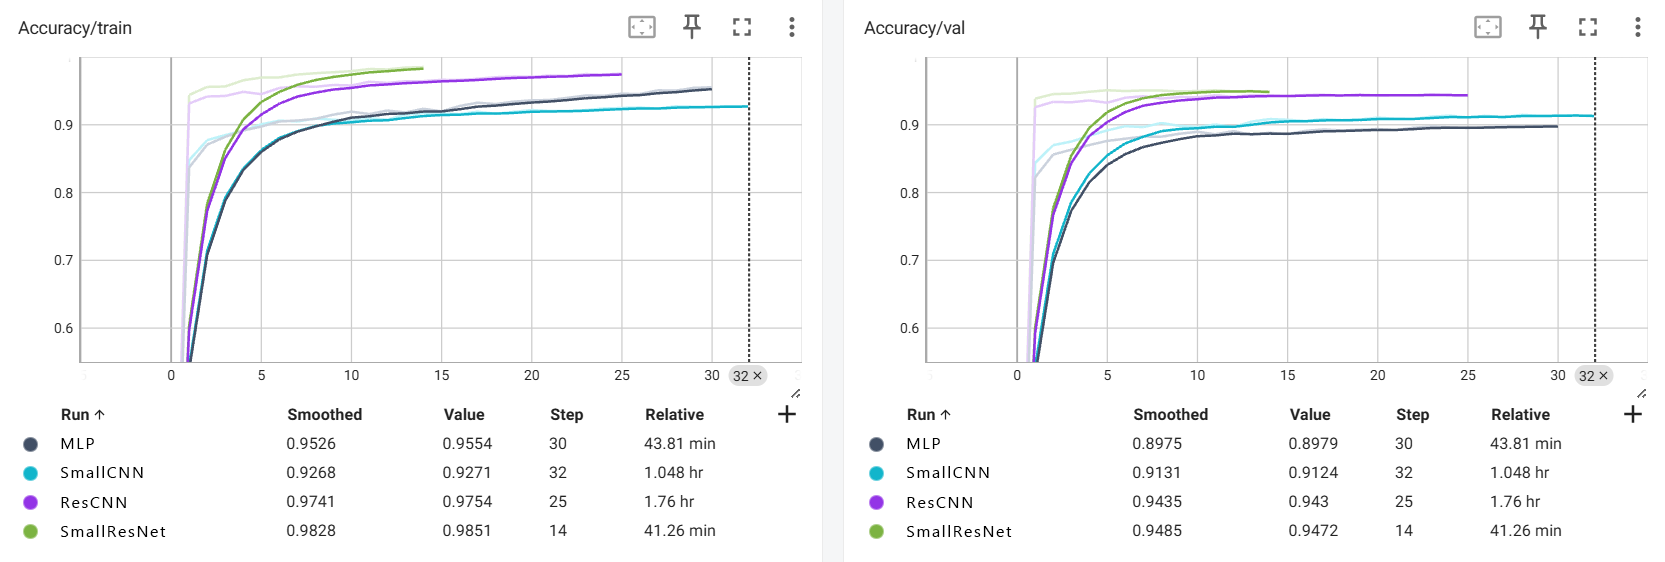
\includegraphics[width=1\textwidth]{tensorboard_accuracy.png}
	\caption{Accuracy}
	\label{accuracy}
\end{figure}

输出模型在验证集、测试集的准确率、loss如表1。
\begin{table}[!ht]
    \begin{center}
        \begin{tabular}{|r|c|c|c|c|}
            \hline
            \multirow{2}{*}{\textbf{Model}} & \multicolumn{2}{c|}{\textbf{Validation}} & \multicolumn{2}{c|}{\textbf{Test}}\\
            \cline{2-5}
            ~ & \textbf{Accuracy} & \textbf{Loss} & \textbf{Accuracy} & \textbf{Loss} \\
            \hline
            \textbf{MLP} & 0.89763 & 0.045164 & 0.90038 & 0.04607 \\ \hline
            \textbf{SmallCNN} & 0.91478 & 0.039486 & 0.91553 & 0.03975 \\ \hline
            \textbf{ResCNN} & 0.94423 & 0.034856 & 0.94409 & 0.03511 \\ \hline
            \textbf{SmallResNet} & 0.95100 & 0.031972 & 0.94779 & 0.03377 \\ \hline
        \end{tabular}
        \caption{Accuracy and Loss}
        \label{tab:results}
    \end{center}
\end{table}

由实验结果可见:
\begin{itemize}
\item 当在CNN中添加了具有跳跃连接的残差块时,准确率的提升最大,达到了约0.03;其次是在基础MLP模型上添加卷积、BN等层,可以使准确率提升约0.015。
\item MLP在达到约10个epoch时,验证集上的准确率不再提高,而在测试集上的准确率仍然缓慢提高,推测出现了过拟合。
\item ResCNN的参数量明显小于SmallResNet,但是其在测试集上的准确率只相差0.004左右,这可能是由于EMNIST数据集仅为灰阶图片,不需要太多参数即可达到较高准确率。
\end{itemize}

四次实验的混淆矩阵如图2。
\begin{figure}[!ht]
    \centering
    \begin{subfigure}{0.45\textwidth}
        \centering
        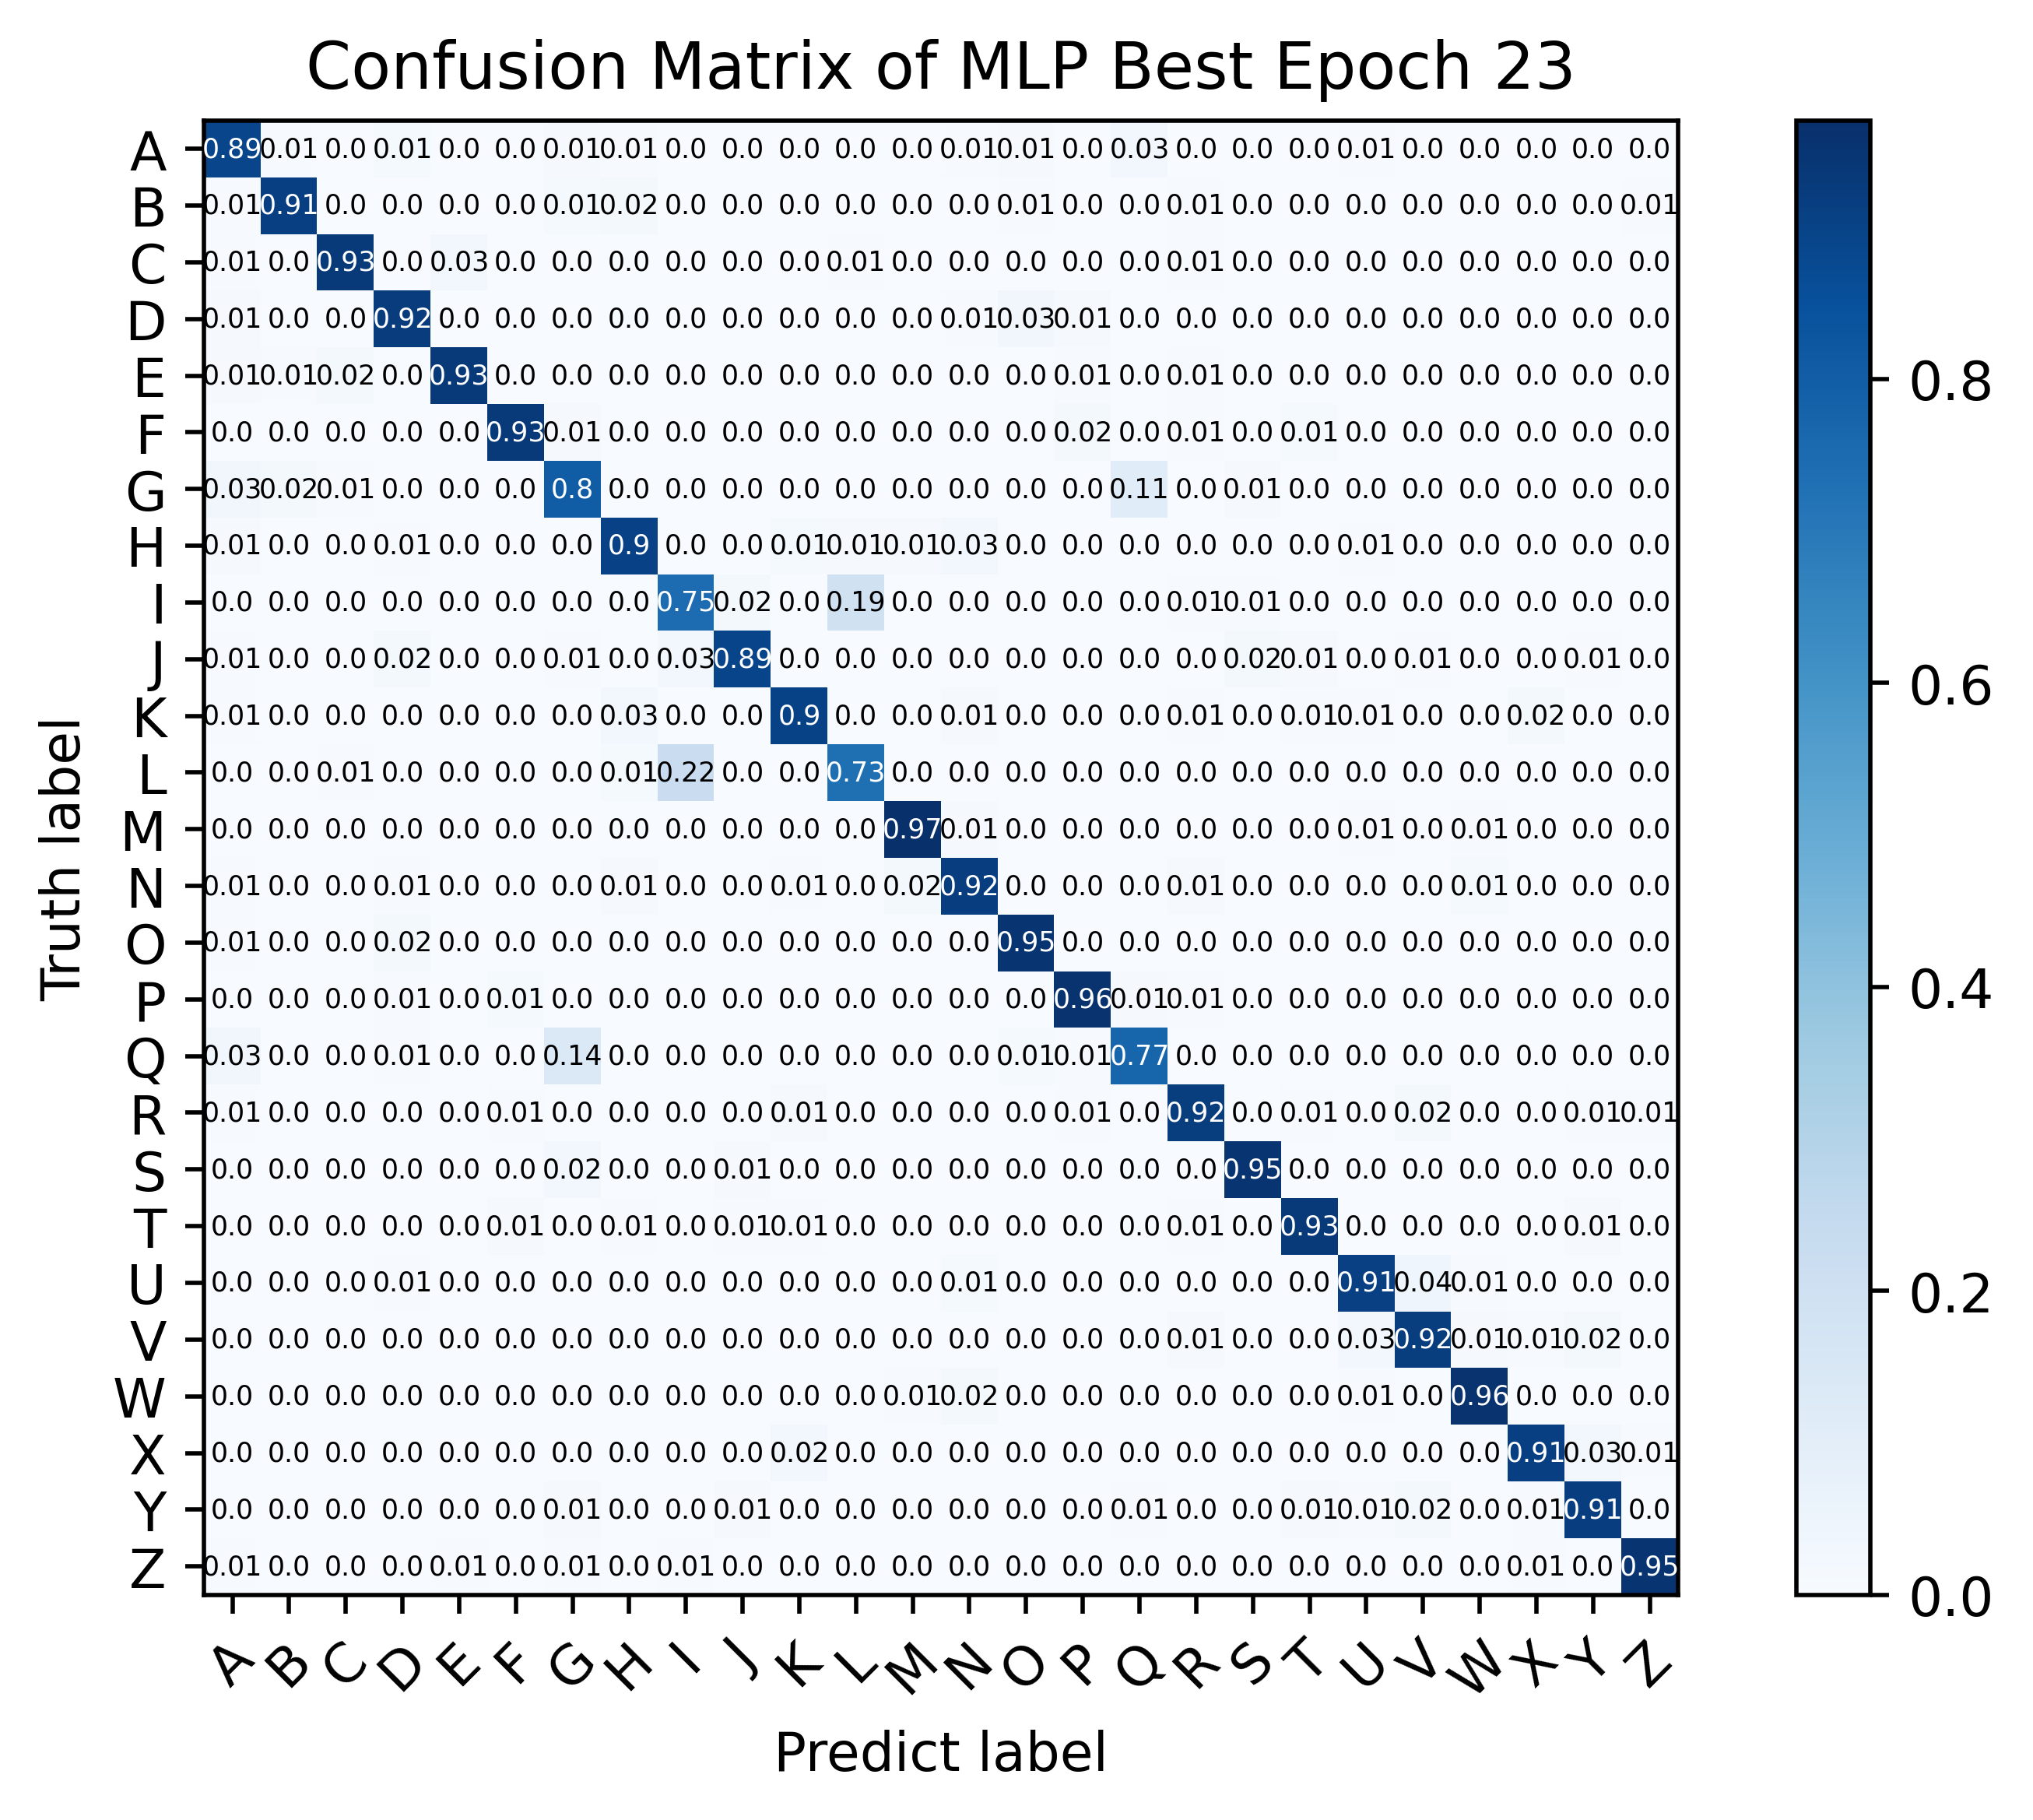
\includegraphics[width=\linewidth]{confusion_matrix_mlp.png}
        \caption{MLP}
        \label{fig:sub1}
    \end{subfigure}
    \hfill
    \begin{subfigure}{0.45\textwidth}
        \centering
        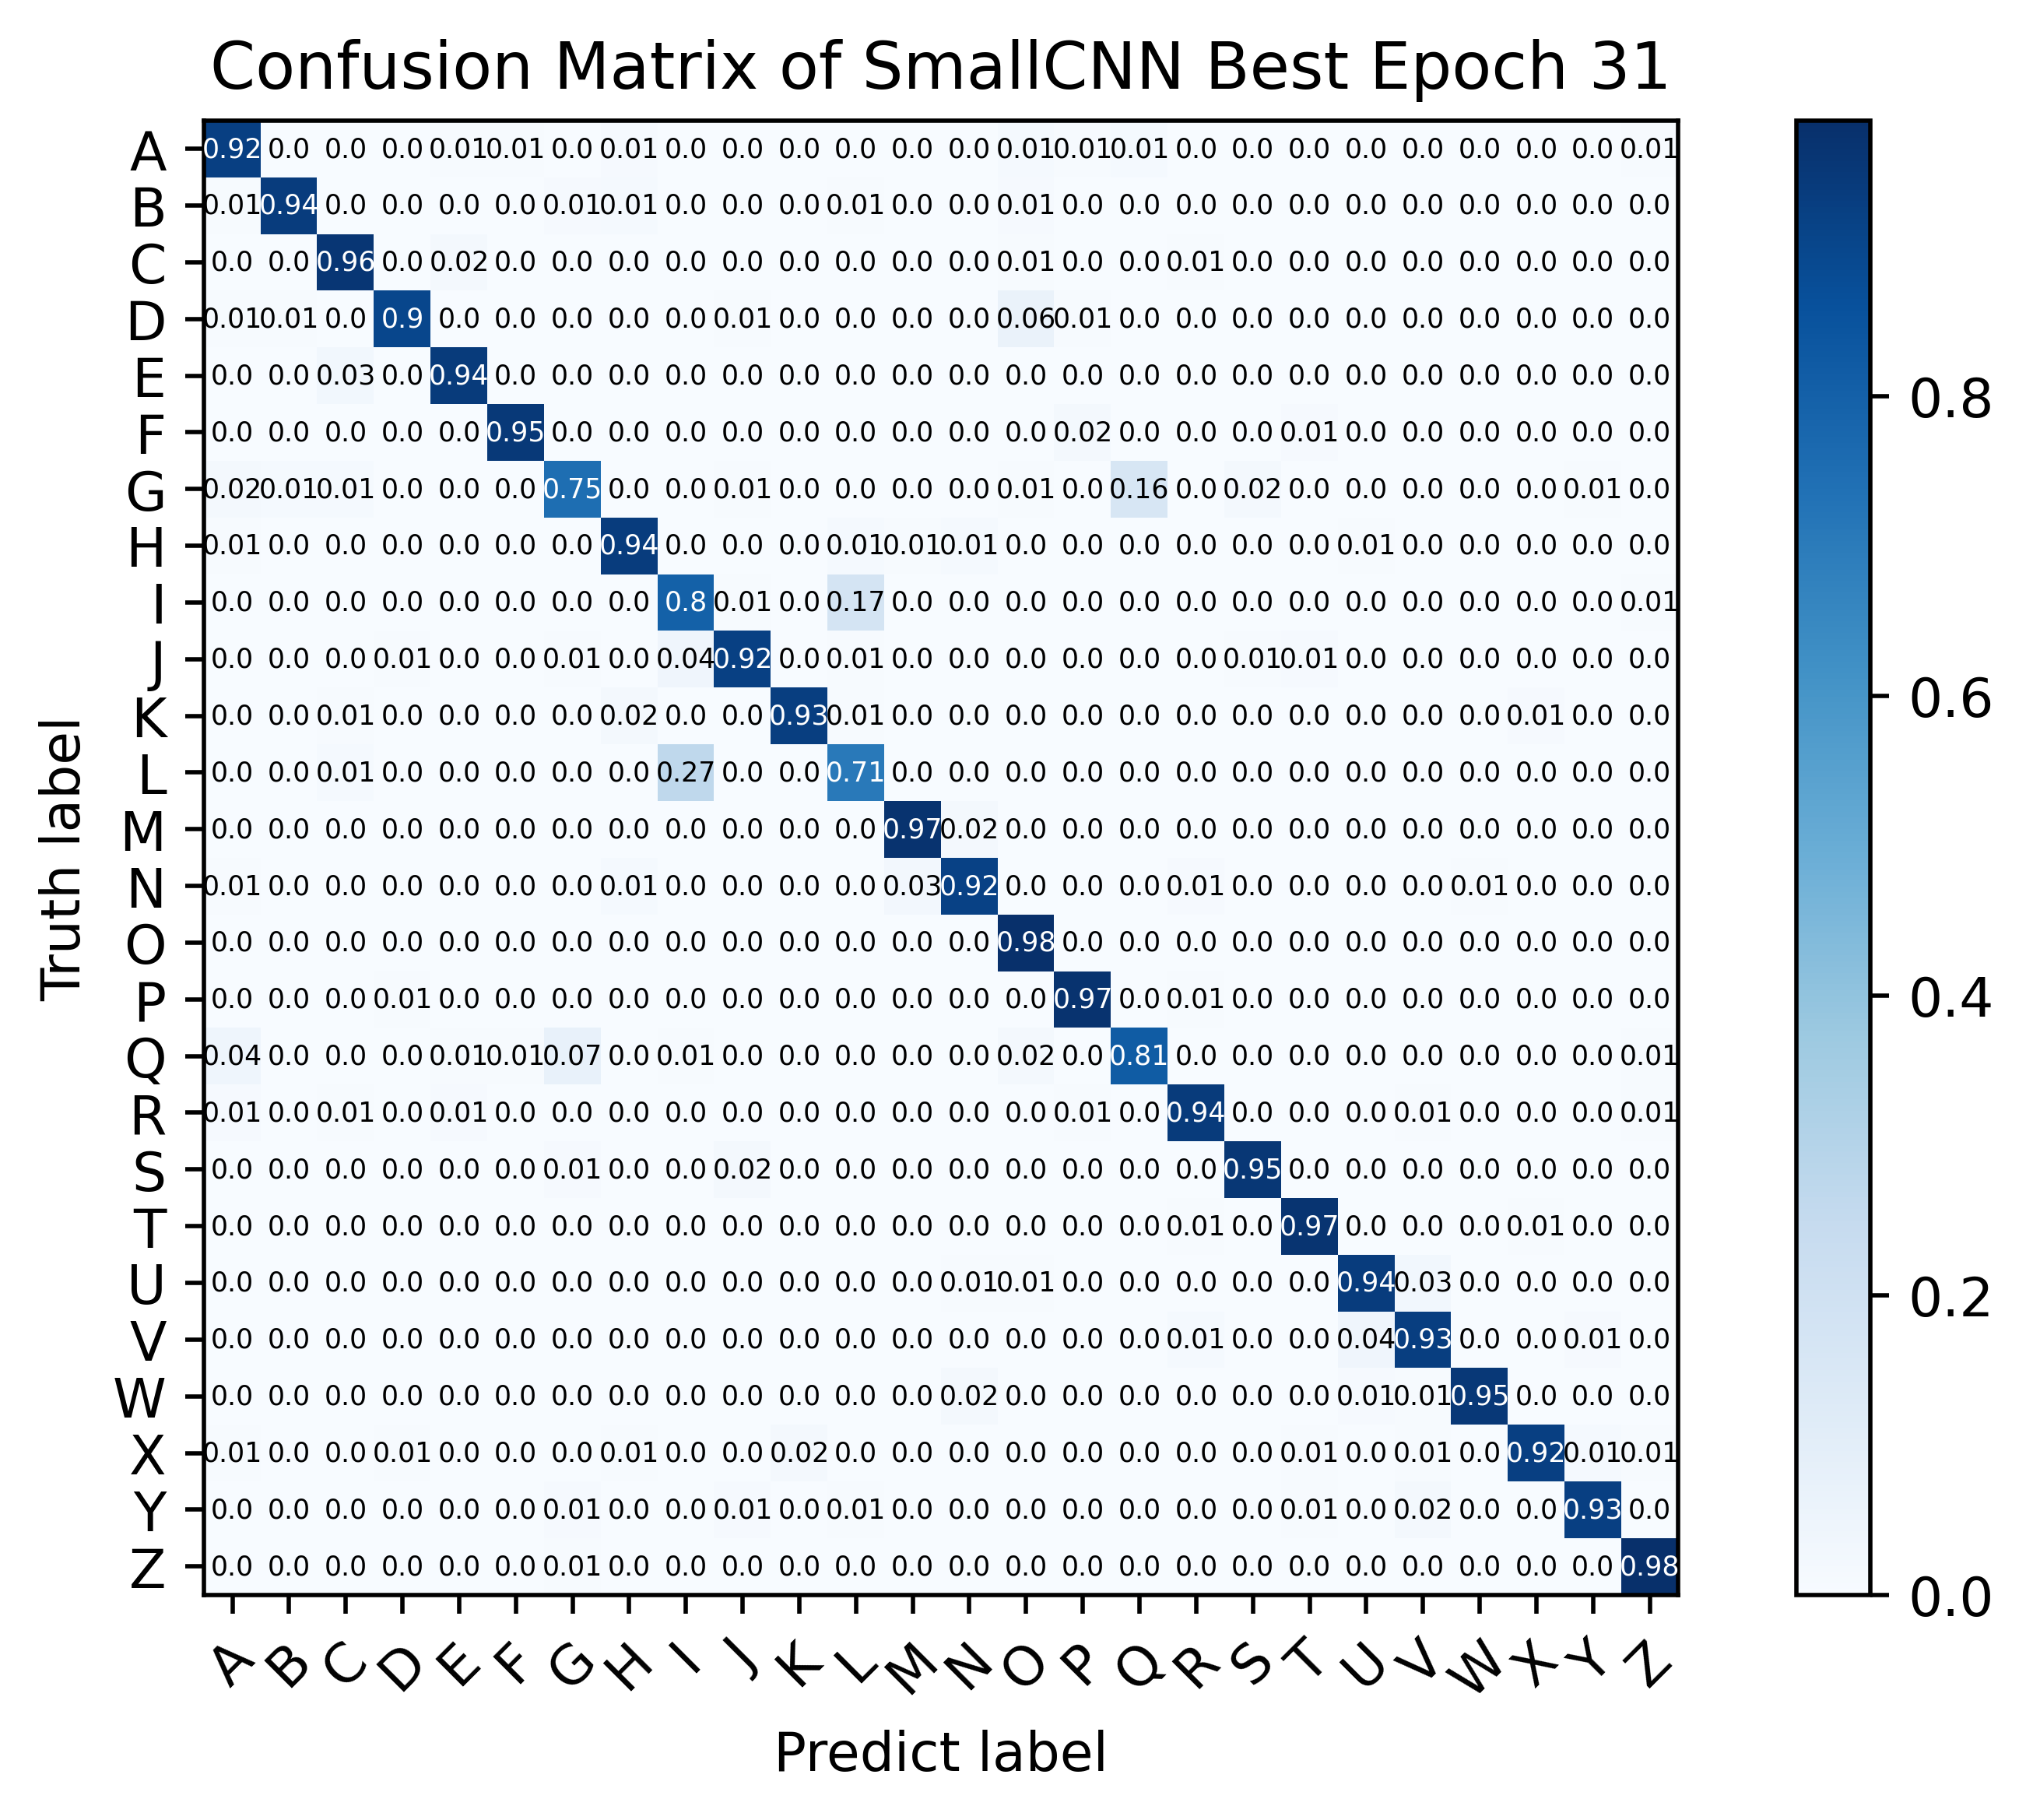
\includegraphics[width=\linewidth]{confusion_matrix_smallcnn.png}
        \caption{SmallCNN}
        \label{fig:sub2}
    \end{subfigure}
    
    \begin{subfigure}{0.45\textwidth}
        \centering
        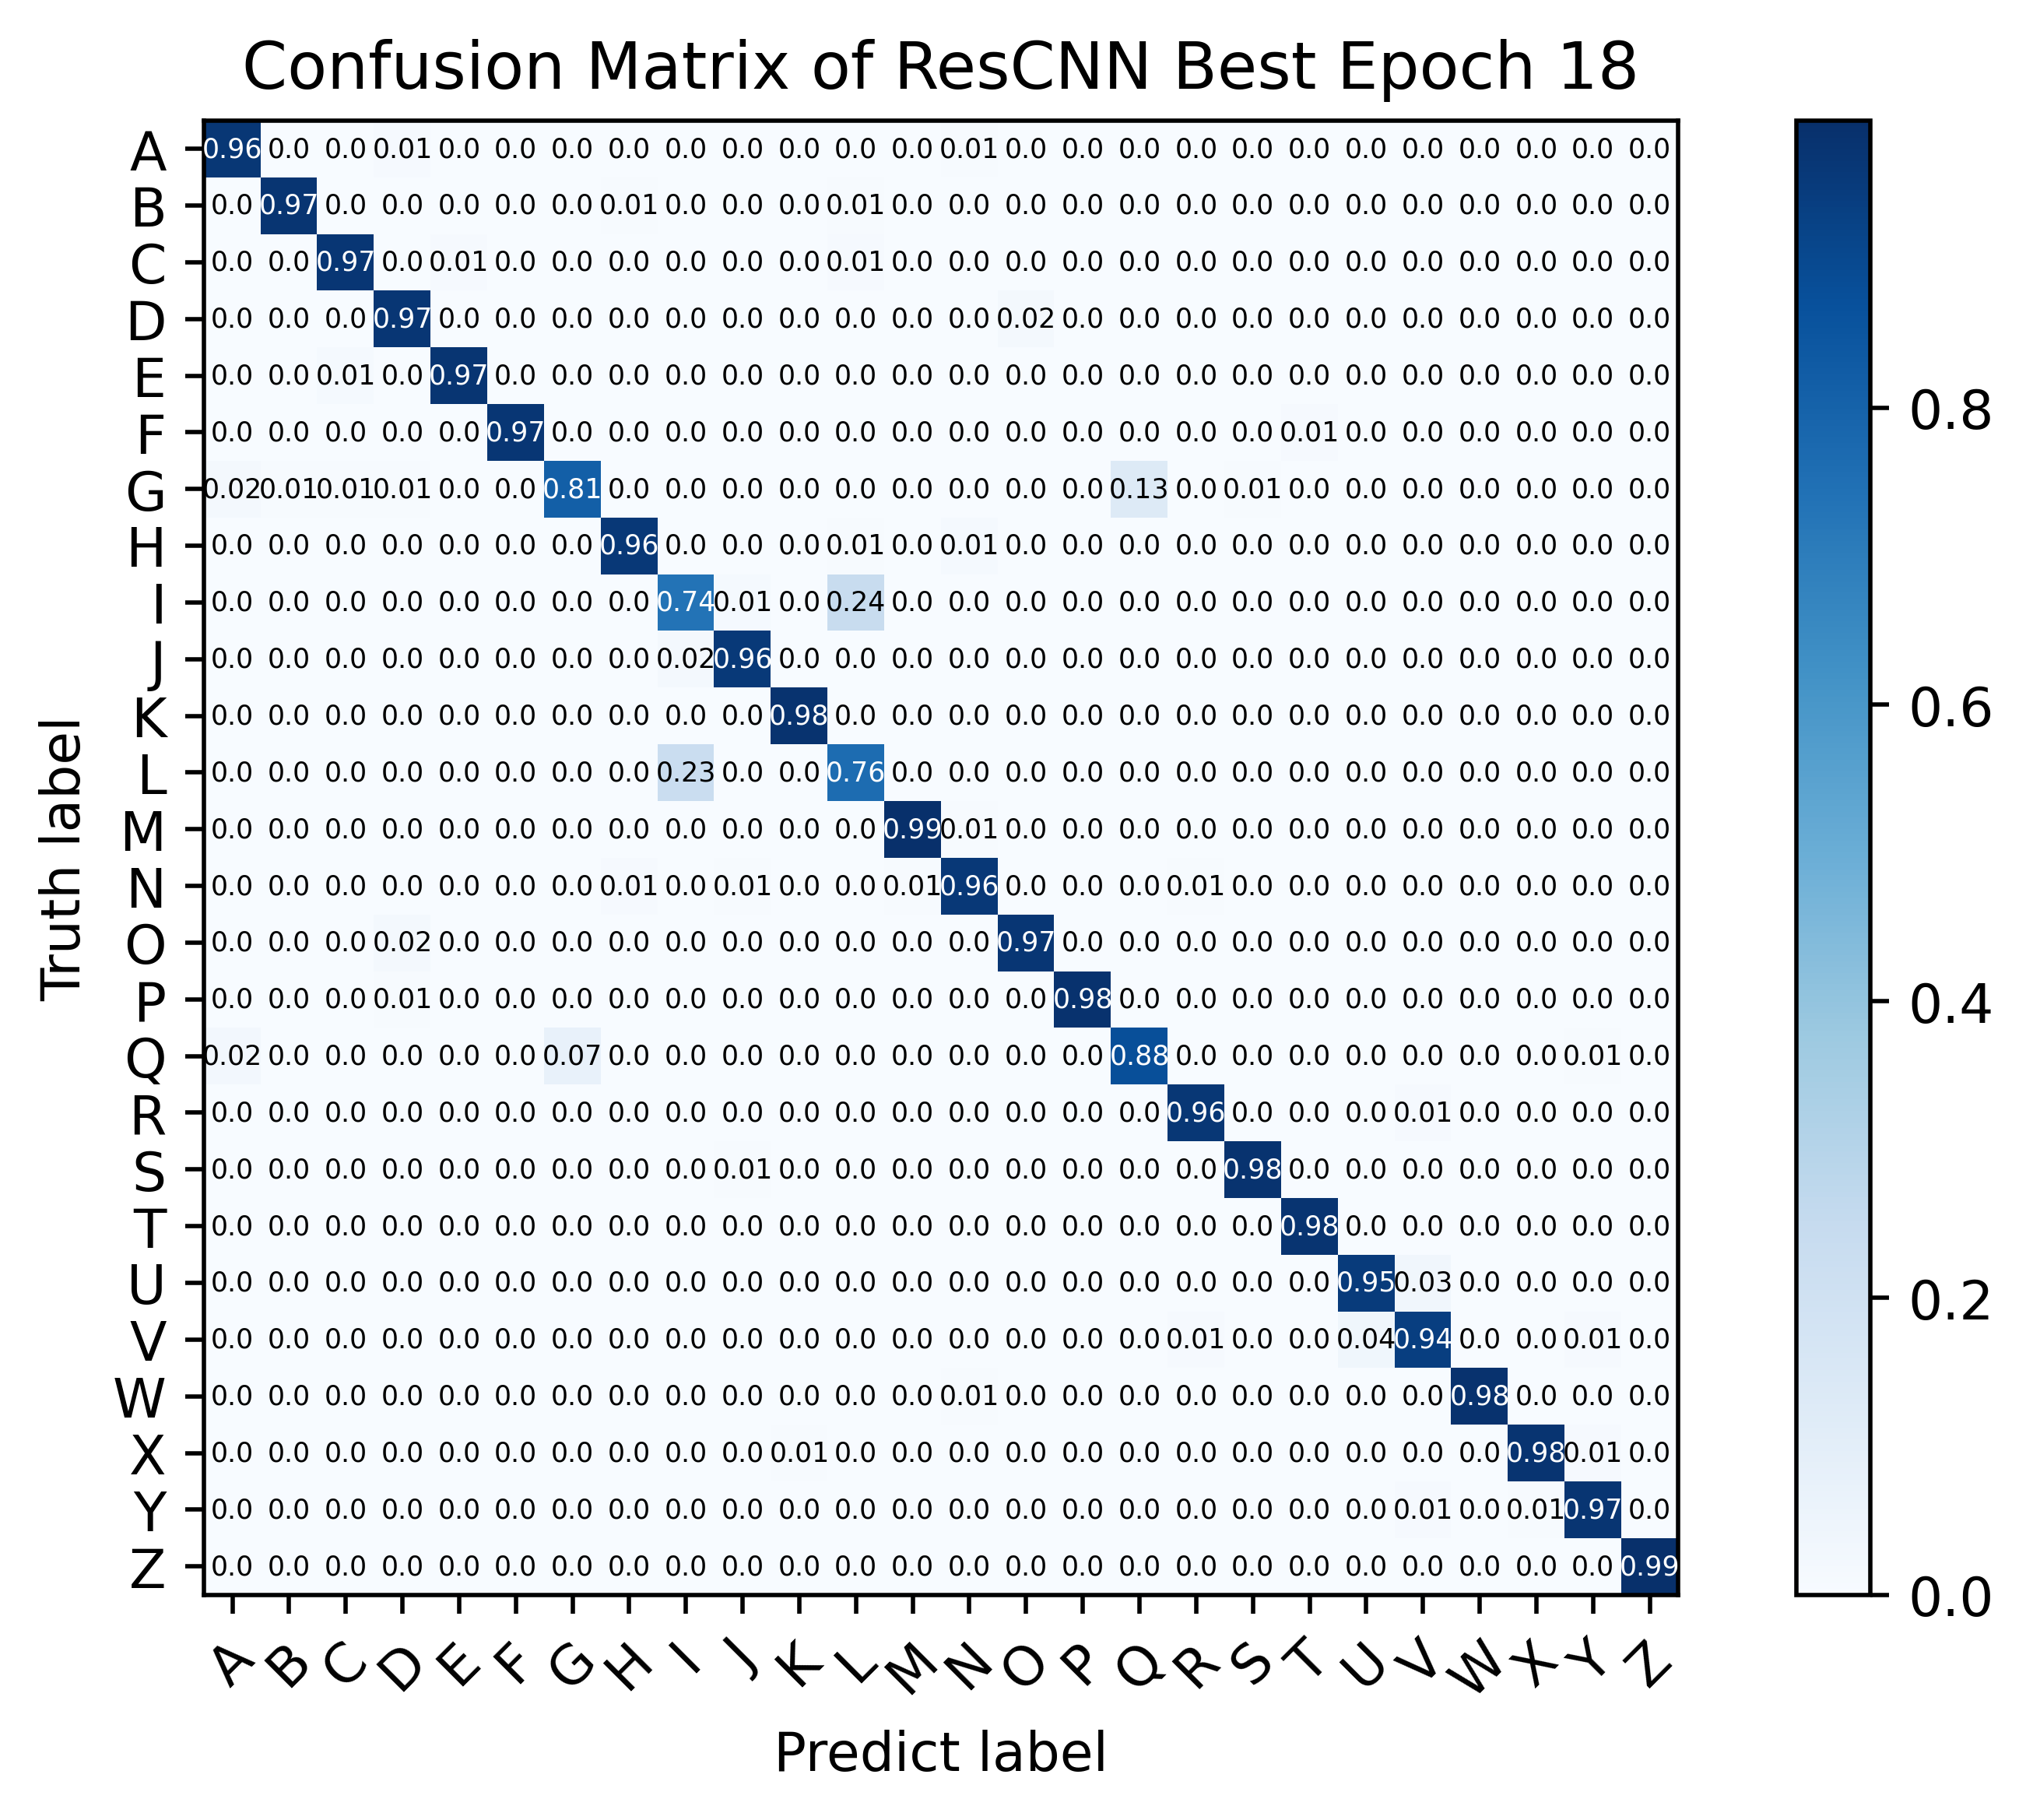
\includegraphics[width=\linewidth]{confusion_matrix_rescnn.png}
        \caption{ResCNN}
        \label{fig:sub3}
    \end{subfigure}
    \hfill
    \begin{subfigure}{0.45\textwidth}
        \centering
        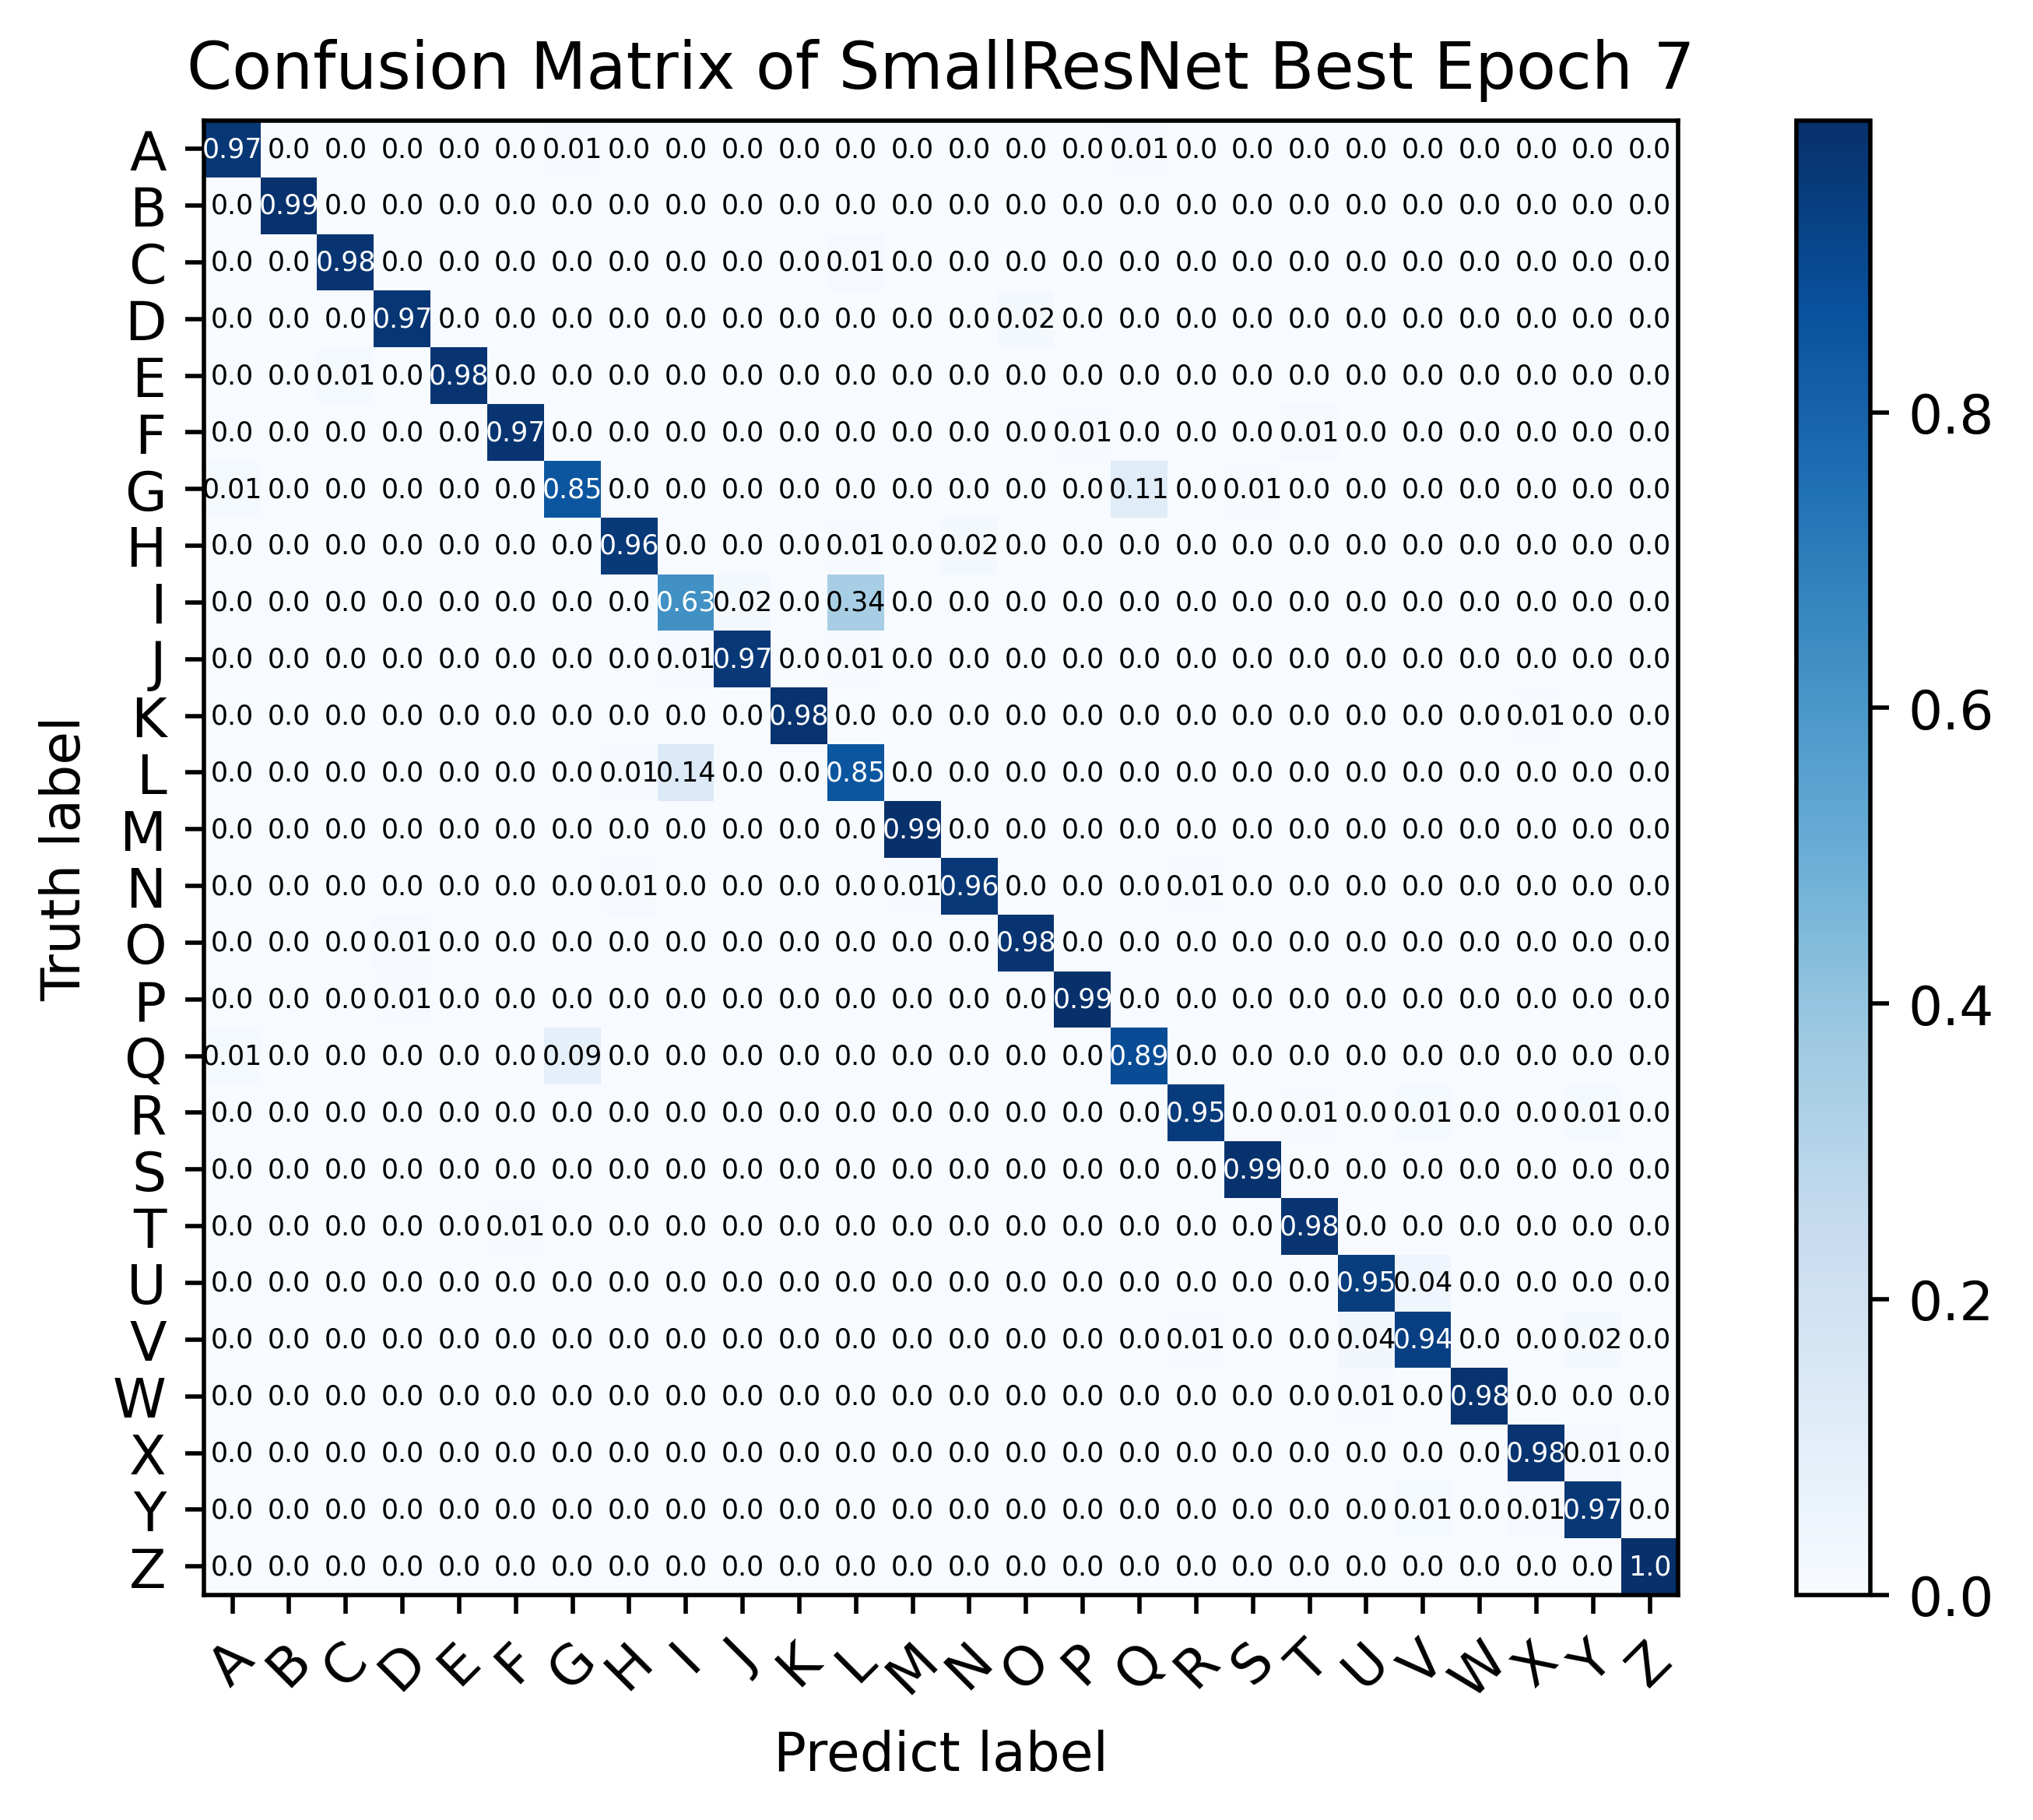
\includegraphics[width=\linewidth]{confusion_matrix_smallresnet.png}
        \caption{SmallResNet}
        \label{fig:sub4}
    \end{subfigure}
    
    \caption{Confusion Matrix}
    \label{fig:confusion_matrix}
\end{figure}

整理所有错误率在0.1以上的结果为表2。
\begin{table}[!ht]
    \centering
    \begin{tabular}{|r|c|c|c|c|c|c|c|c|c|c|c|c|c|}
    \hline
        \textbf{Model} & \multicolumn{4}{c|}{\textbf{MLP}} & \multicolumn{3}{c|}{\textbf{SmallCNN}} & \multicolumn{3}{c|}{\textbf{ResCNN}} & \multicolumn{3}{c|}{\textbf{SmallResNet}} \\ \hline
        \textbf{Truth} & L & I & Q & G & L & I & G & I & L & G & I & L & G \\ \hline
        \textbf{Predict} & I & L & G & Q & I & L & Q & L & I & Q & L & I & Q \\ \hline
        \textbf{Possibility} & 0.22 & 0.19 & 0.14 & 0.11 & 0.27 & 0.17 & 0.16 & 0.24 & 0.23 & 0.13 & 0.34 & 0.14 & 0.11 \\ \hline
    \end{tabular}
    \caption{Results with Error Rate over 0.1}
    \label{tab:results}
\end{table}

可见,现在仍存在的最容易混淆的是I和L,其次是Q和G。在字形上,这两对字母比较相似,错误概率高属于正常现象。但是,注意到SmallResNet上I误判成L的概率达到了0.34,明显高于其他模型,这有待进一步实验来确认原因。

\section{计划}

\iffalse
关于下周的计划,我现在有几种设想:
\begin{itemize}
\item 继续基于EMNIST数据集,对当前的ResCNN与SmallResNet模型进行优化与超参数的调整,使模型的准确率达到0.95以上。
\item 继续基于EMNIST数据集,但使用更加现代的模型如ViT等,使模型的准确率达到0.95以上。但由于EMNIST数据集为灰度图像、分辨率较小和数据量较少,可能不足以支撑ViT模型的训练与测试。
\item 放弃使用EMNIST,迁移到ImageNet等较大数据集上进行更现代的模型的训练。
\end{itemize}
\fi

基于当前的混淆矩阵,我下周的计划是对当前的模型进行优化并调整相应超参数,尝试引入attention机制,使模型的准确率达到0.95以上。

\end{document}